% !TEX root = platooning.tex
\section{Scenario Case Study \label{sec:scenarios}}
In this section, we consider several situations that quadrotors in a platoon on an air highway may commonly encounter, and show via simulations the behaviors that emerge from the controllers we defined in Sections \ref{sec:liveness} and \ref{sec:safety}.

\subsection{Forming a Platoon}
We first consider the scenario in which some quadrotors are trying to merge onto an initially unoccupied highway. In order to do this, each quadrotor first checks for safety with respect to the other quadrotors, and uses the safety controller if necessary, according to Section \ref{sec:safety}. Otherwise, the quadrotor uses the liveness controller described in Section \ref{sec:liveness}. 

For the simulation example, the highway is specified by the line $p_y = 0.5p_x$, the point of entry on the highway is chosen to be $(\bar{p}_x, \bar{p}_y) = (4,2)$, and the target velocity is such that the quadrotors travel at a speed $\bar{v}=3$ along the direction of the highway. This forms the target state $\bar{x}_H=(\bar{p}_x, \bar{v}_x, \bar{p}_y, \bar{v}_y)$, from which we define the target set $\mathcal{L}_H$ as in Section \ref{subsec:highway_merge}.

The first quadrotor that completes merging onto the empty highway creates a platoon and becomes its leader, while subsequent quadrotors form a platoon behind the leader in a pre-specified order according to the process described in Section \ref{subsec:platoon_merge}. Here, we choose $(\bar{p}_{x,r}, \bar{p}_{y,r})$ to be a distance $b$ behind the last quadrotor in the platoon, and $(\bar{v}_{x,r}, \bar{v}_{y,r}) = (0,0)$. This gives us the target set $\mathcal{L}_P$.

Figures \ref{fig:normal2} and \ref{fig:normal5} show the simulation results. Since the liveness reachable sets are in 4D and the safety reachable sets are in 6D, we compute and plot their 2D slices based on the quadrotors' velocities and relative velocities. 

Figure \ref{fig:normal2} illustrates the use of liveness and safety reachable sets using just two quadrotors to reduce visual clutter. The first quadrotor $Q_1$ (red disk) first travels in a straight line towards the highway merging point $\bar{x}$ (red circle) at $t=1.5$, because it is not yet in the liveness reachable set for merging onto the highway (red dotted boundary). When it is within the liveness reachable set boundary at $t=2.8$, it is ``locked-in" to the target state $\bar{x}_H$, and follows the optimal control in \eqref{eq:HJB_ctrl_syn} to $\bar{x}_H$. During the entire time, $Q_1$ checks whether it may collide with $Q_2$ within a time horizon of $t_\text{external}$; we chose $t_\text{external}=3>t_\text{internal}$. 

After $Q_1$ has reached $\bar{x}_H$, it forms a platoon, becomes the platoon leader, and continues to travel along the highway. $Q_2$ (blue disk), at $t=7$, begins joining the platoon behind $Q_1$, by moving towards the target $\bar{x}_P$ relative to the position of $Q_1$. When $Q_2$ moves inside the liveness reachable set boundary for joining the platoon (blue dotted boundary), it is ``locked-in" to the target relative state $\bar{x}_P$, and begins following the optimal control in \eqref{eq:HJI_ctrl_syn} towards the target whenever it is outside the safety reachable set (blue dashed boundary).

Figure \ref{fig:normal5} shows the behavior of all 5 quadrotors which eventually form a platoon and travel along the highway together. The liveness controllers allow the quadrotors to optimally and smoothly enter the highway and join platoons, while the safety controllers prevent collisions from occurring.

\begin{figure}
	\centering
	\includegraphics[width=0.35\textwidth]{"fig/normal2"}
	\caption{Reachable sets used to merge onto a highway to form a platoon (top subplots) and to join a platoon on the highway (bottom subplots).}
	\label{fig:normal2}
\end{figure}

\begin{figure}
	\centering
	\includegraphics[width=0.35\textwidth]{"fig/normal5"}
	\caption{Five quadrotors merging onto a highway.}
	\label{fig:normal5}
\end{figure}

\subsection{Malfunctioning Vehicle in Platoon}
We now consider a scenario where a quadrotor in a platoon of five malfunctions while the platoon is traveling along a highway. To best demonstrate the behavior of the other quadrotors in the platoon, this simulation assumes that $Q_{P_3}$, the middle quadrotor, malfunctions and reverses direction. When this happens, all of the other quadrotors in the platoon begin checking safety against it. In addition, $Q_{P_3}$ is removed from the platoon, causing the other quadrotors to treat it as an intruder.  Trailing quadrotors must leave the highway to avoid colliding with the faulty quadrotor. 

Figure \ref{fig:faulty2} shows the platoon of quadrotors, $Q_i,i = 1,...,5$ with $P_i = i$, traveling along the highway. At $t=0, Q_3$ malfunctions and begins to track the highway in reverse. Once $Q_3$ malfunctions, it is removed from the platoon and treated as an intruder. The platoon is then restructured with the faulty quadrotor removed ($Q_{P_i} = Q_{i+1}$ for $i=3,4$). After avoiding $Q_3$, the trailing quadrotors $Q_4$ and $Q_5$ accelerate to reach their new platoon positions. $Q_1$ and $Q_2$ are unaffected by the malfunctioning quadrotor. 

Figure \ref{fig:faulty2} also shows the safe reachable set of $Q_4$ with respect to $Q_3$ (green dashed line), and the safe reachable set of $Q_5$ with respect to $Q_4$ and $Q_3$ (purple dashed lines).

At $t=1,Q_4$ applies the safe controller to avoid entering the safe reachable set with respect to $Q_3$. During $Q_4$'s avoidance maneuver, $Q_5$ simply follows $Q_4$, and does not come across any safety breaches, as shown by the $t=1$ and $t=2.1$ subplots. The safety breach ends soon after, and by $t=4.5$, $Q_4$ begins merging back onto the highway, followed by $Q_5$, in order to continue to follow the platoon. In this particular case, the safety breach is resolved even without any altitude change.

%\begin{figure}
%	\center
%		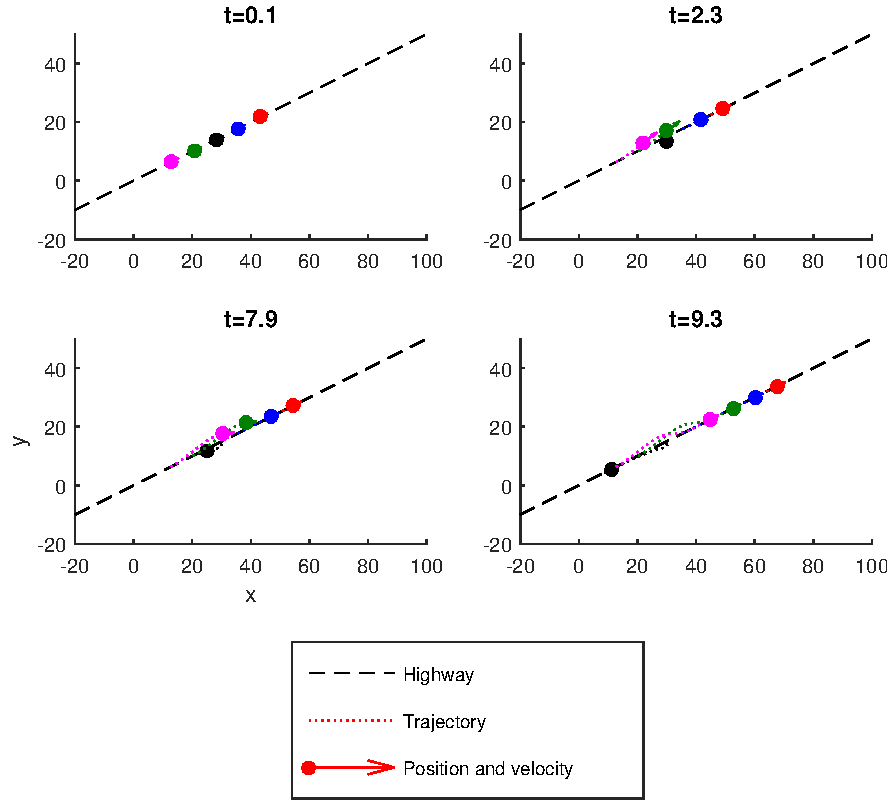
\includegraphics[width=0.45\textwidth]{fig/faultyNoRsets}
%		\caption{A quadrotor in the platoon becomes faulty. The rest of the platoon safely avoids the quadrotor and continues normal operation as a platoon once the faulty quadrotor has been cleared.}
%		\label{fig:faulty1}
%\end{figure}

\begin{figure}
	\center
		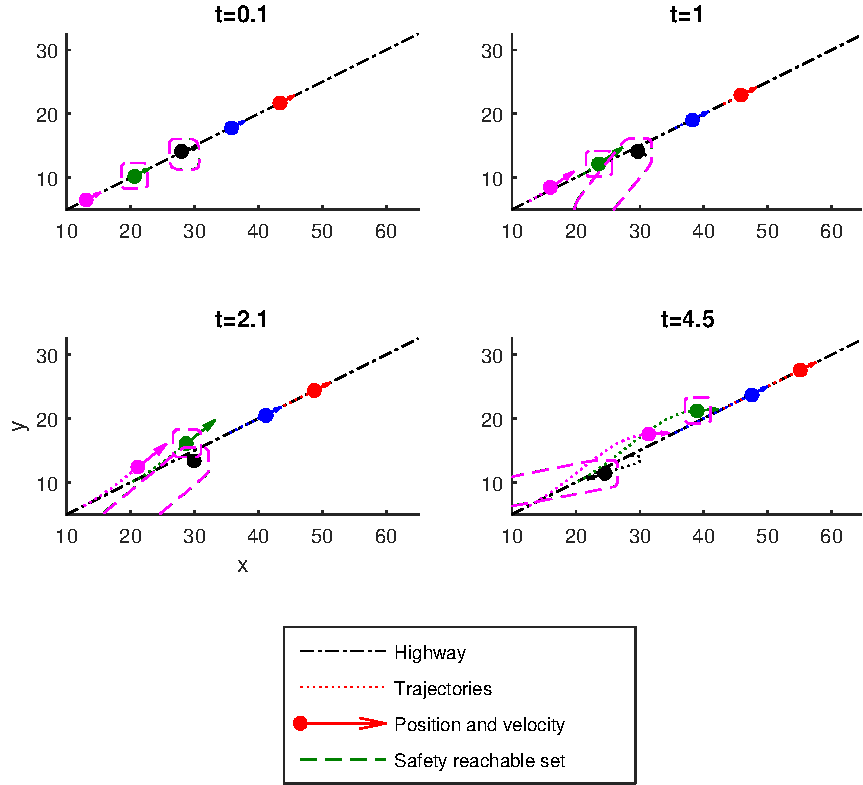
\includegraphics[width=0.4\textwidth]{fig/faultyRsets}
		\caption{Reachable sets used by trailing quadrotors to avoid colliding with the faulty quadrotor.}
		\label{fig:faulty2}
\end{figure}

\subsection{Intruder Vehicle}
We now consider the scenario in which a platoon of quadrotors encounters an intruder vehicle. To avoid collision, each quadrotor checks for safety with respect to the intruder and any quadrotor in front and behind in the platoon. If necessary, each quadrotor switches to using the safety controller.

Figure \ref{fig:intruder1} shows the simulation result. At $t=0$, a platoon of 4 quadrotors, $Q_{P_i},i=1,\ldots,4$ with $P_i = i$, travel along the highway. An intruder vehicle $Q_0$ (red disk) starts from position $(40,30)$ and heads toward bottom-left of the grid. 

The platoon leader $Q_{P_1}$'s (black disk) safety is unaffected by the intruder. Followers $Q_{P_2}$ (blue disk), $Q_{P_3}$ (green disk) and $Q_{P_4}$ (pink disk), on the other hand, must use the safety controller in order to avoid collision with the intruder ($t=3.3,6.2$). This causes their paths to deviate off the highway. Once each quadrotor is safe relative to the intruder, they rejoin the original platoon ($t=12.4$). Figure \ref{fig:intruder2} illustrates the use of safety reachable sets in this scenario using only $Q_{P_2}$ as an example. The safety reachable sets of $Q_{P_2}$ with respect to the intruder $Q_0$, $Q_{P_1}$ and $Q_{P_3}$ (red, black, green dashed lines) are shown. %With respect to $Q_0$, $Q_{P_2}$'s safety is considered to be breached if $V_S(-t_\text{external},x_{P_2}-x_0) \le 0$. To avoid possible collision with the intruder, $Q_{P_2}$ must remain outside the safety reachable set with respect to the intruder. The same applies to collision avoidance with $Q_{P_1}$ and $Q_{P_3}$. %\textcolor{red}{\sout{Note that safety reachable sets with $Q_{P_1}$ and $Q_{P_3}$ are much smaller than that with the intruder. This is because under normal conditions, vehicles in the same platoon have near-zero relative velocity. For this reason, they may only check possible collisions within the next 1.5 seconds, instead of 3 seconds for vehicles outside of the platoon. This allows vehicles to travel closer together within a platoon and thus increasing throughput on the air highway.}} \textcolor{blue}{The 1.5 seconds is because we made the assumption that malfunctioning vehicles will change altitude within 1.5 seconds.}

Initially, $Q_{P_2}$ ($P_2=2$) is a follower outside all 3 safety reachable sets. At $t=0.6$, $Q_2$ comes to the boundary of the safety set with respect to the intruder and must apply the safety control law to avoid potential future collision. Thus it splits from the original platoon and becomes the leader of a new platoon consisting of itself, $Q_3$ and $Q_4$. $Q_2$ keeps using the safety controller until it is safe with respect to the intruder again at $t=3$. After $t=3$, $Q_2$ is safe to use the liveness controller again to merge back onto the highway and join the original platoon. Note that during the entire time, $Q_2$ maintains safety against the intruder, $Q_1$ and $Q_3$ by always staying outside of all three safety reachable sets.


\begin{figure}
	\centering
	\includegraphics[width=0.35\textwidth]{"fig/Intruder1"}
	\caption{Reaction of a platoon of 4 quadrotors on a highway to an intruder.}
	\label{fig:intruder1}
\end{figure}

\begin{figure}
	\centering
		\includegraphics[width=0.35\textwidth]{"fig/intruder2"}
	\caption{Reachable sets used by quadrotor $Q_2$ to avoid collision with respect to the intruder and quadrotors $Q_1$ and $Q_3$ in front and behind it respectively.}
	\label{fig:intruder2}
\end{figure}

